\documentclass[10pt]{article}

\def\Type{LessonCaelan}
\def\TypeNum{Lesson 13}
\def\TypeTitle{Absolute Extreme Values }
\def\Semester{Fall 2021} %Not Used 
\def\Course{MATH 1190 \& 1210}
\def\Targets{  {\bf\color{RedOrange}A2} }

\usepackage{preambleDJ}

%\usepackage{ragged2e}


%%%%%%%%%%%% BEGIN DOCUMENT %%%%%%%%%%%%%%%
%%%%%%%%%%%% BEGIN DOCUMENT %%%%%%%%%%%%%%%
%%%%%%%%%%%% BEGIN DOCUMENT %%%%%%%%%%%%%%%
%%%%%%%%%%%% BEGIN DOCUMENT %%%%%%%%%%%%%%%
%%%%%%%%%%%% BEGIN DOCUMENT %%%%%%%%%%%%%%%




\begin{document}

\pagestyle{otherpages}
\thispagestyle{firstpage}
\vs{.3}

\textbf{Intended Learning Outcomes}
After this lesson, you will be able to 

\begin{itemize}
    \item Define absolute extrema and describes its difference from local extrema. (\target{A2})
    \item Apply the Close Interval Method to find the absolute extra of a function in a given close interval. (\target{A2})
    \item Apply the First Derivative Test for Absolute Extrema to find absolute extrema on non-closed intervals. (\target{A2})
\end{itemize}

\vspace{-0.5cm}

\hrulefill\\

\blue{\bf Mini-Lecture and Definitions: }
\tasksI{2}{
\task A {\em Local Maximum} occurs at a critical number $c$ where $$f(x)\leq f(c)$$ for all $x$ ``close" to $c$.
\task A {\em Local Minimum} occurs at a critical number $c$ where  $$f(x)\geq f(c)$$ for all $x$ ``close" to $c$. \vs{.2}
\task An {\em Absolute Maximum} occurs on an interval \\$I=[a,b]$ when we can find a $c$ in $I$ so that  $$f(x)\leq f(c)$$ for all $x$ in $I$.
\task An {\em Absolute Minimum} occurs on an interval \\$I=[a,b]$ when we can find a $c$ in $I$ so that  $$f(x)\geq f(c)$$ for all $x$ in $I$.
}

\blue{\bf Warmup Example/Exercise} For each graph below, identify the number Absolute Max/Mins on the interval $I=[a,b]=[1,4]$. Identify the number of Local Max/Mins on the same interval.\\
\mpageTfour{.35}{.2}{.35}{.2}{
\begin{flushleft}
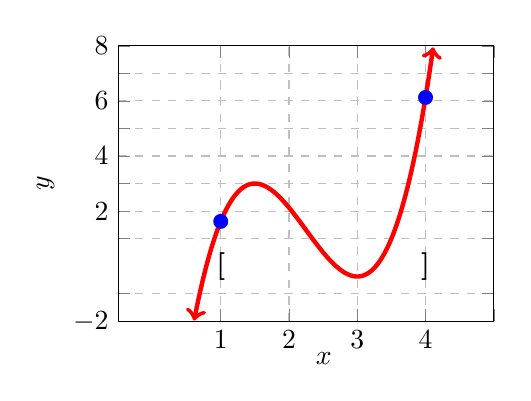
\begin{tikzpicture}[scale=1]
          \begin{axis}[
            xlabel={$x$},
            xlabel style={anchor=west},
            ylabel={$y$}, 
            ylabel style={anchor=south},
            %grid = major,
            xtick       = {1,2,3,4,5},
            xticklabels = {$1$,$2$,$3$,$4$},
            ytick       = {-2,-1,1,2,3,4,5,6,7,8},
            yticklabels = {$-2$,,,$2$,,$4$,,$6$,,$8$},
            samples     = 320,
            domain      = -.5:5,
            restrict y to domain=-2:8,
            xmin = -.5, xmax = 5,
            ymin = -2, ymax = 8,
            grid=both, grid style=dashed,
            height=2in, width=2.5in
          ]
          \addplot[domain=.51:4.5, ultra thick, red,<->] {  2*(x-1.5)^2*(x-3.75)+3  };
          \filldraw[blue] (1,1.625) circle (2.5pt);
          \filldraw[blue] (4,6.125) circle (2.5pt);
          \draw (1,0) node {  \blue{\textbf{[}} };
           \draw (4,0) node {  \blue{\textbf{]}} };
          %
        \end{axis}
    \end{tikzpicture}
    \end{flushleft}
    }{
\hs{.1}\# Local Mins \vs{.3}\\
\hs{.1}\# Local Maxs\vs{.3}\\
\hs{.1}\# Abs Mins \vs{.3}\\
\hs{.1}\# Abs Maxs
}{
\begin{flushleft}
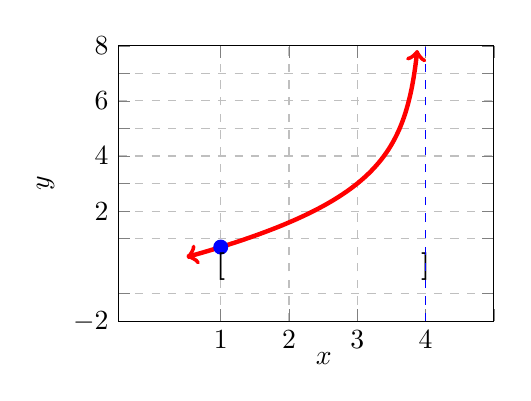
\begin{tikzpicture}[scale=1]
          \begin{axis}[
            xlabel={$x$},
            xlabel style={anchor=west},
            ylabel={$y$}, 
            ylabel style={anchor=south},
            %grid = major,
            xtick       = {1,2,3,4,5},
            xticklabels = {$1$,$2$,$3$,$4$},
            ytick       = {-2,-1,1,2,3,4,5,6,7,8},
            yticklabels = {$-2$,,,$2$,,$4$,,$6$,,$8$},
            samples     = 320,
            domain      = -.5:5,
            restrict y to domain=-2:8,
            xmin = -.5, xmax = 5,
            ymin = -2, ymax = 8,
            grid=both, grid style=dashed,
            height=2in, width=2.5in
          ]
          \addplot[domain=.5:4, ultra thick, red,<->] {  x/(4-x)^(1/3)  };
          \filldraw[blue] (1,.6933) circle (2.5pt);
%          \filldraw[blue] (4,6.125) circle (2.5pt);
          \draw (1,0) node {  \blue{\textbf{[}} };
           \draw (4,0) node {  \blue{\textbf{]}} };
           \draw[dashed, blue] (4,-2) -- (4,9);
          %
        \end{axis}
    \end{tikzpicture}
    \end{flushleft}
}{
\hs{.1}\# Local Mins \vs{.3}\\
\hs{.1}\# Local Maxs\vs{.3}\\
\hs{.1}\# Abs Mins \vs{.3}\\
\hs{.1}\# Abs Maxs
}
~\\
\mpageTfour{.35}{.2}{.35}{.2}{
\begin{flushleft}
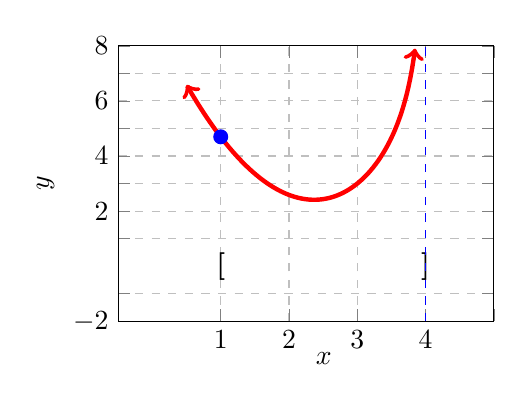
\begin{tikzpicture}[scale=1]
          \begin{axis}[
            xlabel={$x$},
            xlabel style={anchor=west},
            ylabel={$y$}, 
            ylabel style={anchor=south},
            %grid = major,
            xtick       = {1,2,3,4,5},
            xticklabels = {$1$,$2$,$3$,$4$},
            ytick       = {-2,-1,1,2,3,4,5,6,7,8},
            yticklabels = {$-2$,,,$2$,,$4$,,$6$,,$8$},
            samples     = 320,
            domain      = -.5:5,
            restrict y to domain=-2:8,
            xmin = -.5, xmax = 5,
            ymin = -2, ymax = 8,
            grid=both, grid style=dashed,
            height=2in, width=2.5in
          ]
          \addplot[domain=.5:4, ultra thick, red,<->] {  x/(4-x)^(1/3)+(x-3)^2 };
          \filldraw[blue] (1,4.696) circle (2.5pt);
%          \filldraw[blue] (4,6.125) circle (2.5pt);
          \draw (1,0) node {  \blue{\textbf{[}} };
           \draw (4,0) node {  \blue{\textbf{]}} };
             \draw[dashed, blue] (4,-2) -- (4,9);
          %
        \end{axis}
    \end{tikzpicture}
    \end{flushleft}
}{
\hs{.1}\# Local Mins \vs{.3}\\
\hs{.1}\# Local Maxs\vs{.3}\\
\hs{.1}\# Abs Mins \vs{.3}\\
\hs{.1}\# Abs Maxs
}{
\begin{flushleft}
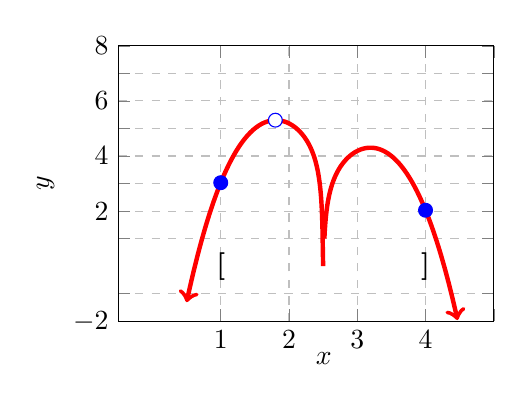
\begin{tikzpicture}[scale=1]
          \begin{axis}[
            xlabel={$x$},
            xlabel style={anchor=west},
            ylabel={$y$}, 
            ylabel style={anchor=south},
            %grid = major,
            xtick       = {1,2,3,4,5},
            xticklabels = {$1$,$2$,$3$,$4$},
            ytick       = {-2,-1,1,2,3,4,5,6,7,8},
            yticklabels = {$-2$,,,$2$,,$4$,,$6$,,$8$},
            samples     = 320,
            domain      = -.5:5,
            restrict y to domain=-2:8,
            xmin = -.5, xmax = 5,
            ymin = -2, ymax = 8,
            grid=both, grid style=dashed,
            height=2in, width=2.5in
          ]
          \addplot[domain=.5:2.49, ultra thick, red,<-] {  (x-5/2)^3+ln(5/2-x)+6  };
           \addplot[domain=2.5183:4.5, ultra thick, red,->] {  -(x-5/2)^3+ln(x-5/2)+5  };
           \draw[ultra thick, red] (2.49,1.39) -- (2.5,0);
          \filldraw[blue] (1,3.03) circle (2.5pt);
          \filldraw[blue] (4,2.03) circle (2.5pt);
                   \filldraw[blue, fill=white] (1.8,5.3) circle (2.5pt);
          \draw (1,0) node {  \blue{\textbf{[}} };
         \draw (4,0) node {  \blue{\textbf{]}} };
%           \draw[dashed, blue] (2.5,-2) -- (2.5,9);
          %
        \end{axis}
    \end{tikzpicture}
    \end{flushleft}
}{
\hs{.1}\# Local Mins \vs{.3}\\
\hs{.1}\# Local Maxs\vs{.3}\\
\hs{.1}\# Abs Mins \vs{.3}\\
\hs{.1}\# Abs Maxs
}
~\\
 ({\bf Extreme Value Theorem}) {\bf If} $f$ is {\em continuous} on $[a,b]$, {\bf then} $f$ attains an absolute maximum and minimum somewhere on $[a,b]$
\vs{.3}\\
{\em Key Observations}\vs{.5}
%{\em Practical Tips}

\newpage

{\bf \blue{ Practical Tips:} Closed Interval Method.} To find the absolute maximum value and absolute minimum value of a continuous function $f$ on the closed interval $[a, b]$, do the following:
\smallskip

\begin{minipage}{0.75\textwidth}
\enum{
\item  Find the critical numbers $c_1, c_2, \ldots, c_n$ of $f$ that lie in $(a, b)$.
\item  Find the value of $f$ at each critical number {\em and} at the endpoints


\item  The largest value from $2$)  will be the absolute maximum value of $f$ on $[a, b]$ and the smallest vakye will be the absolute minimum value of $f$ on $[a, b]$. 
}
\end{minipage}
%
\hfill
%
\begin{minipage}{0.2\textwidth}
\begin{center}
\begin{tabular}{|c|c|}
\hline 
$x$ & $f(x)$\tabularnewline
\hline 
\hline 
$a$ & $f(a)$\tabularnewline
\hline 
$b$ & $f(b)$\tabularnewline
\hline 
$c_1$ & $f(c_1)$\tabularnewline
\hline 
$c_2$ & $f(c_2)$\tabularnewline
\hline 
$\vdots$ &$\vdots $\tabularnewline
\hline 
$c_n$ & $f(c_n)$\tabularnewline
\hline 
\end{tabular}
\end{center}
\end{minipage}
 {\example}\ltrm{\color{RedOrange}A2} Find the absolute maximum and absolute minimum values of $f(x)=\sqrt[3]{x^2-4x}$, where $x$ is in $[-1,3]$.

\vfill
 

 

{\exercise}\ltrm{\color{RedOrange}A2} Find the absolute maximum and absolute minimum values of $\ds f(x)=\frac{1}{3}x^3-2x^2+\frac{5}{3}$ on the interval $[-1,1]$.   
    \vfill

\newpage
    
{\exercise}\ltrm{\color{RedOrange}A2} Find the absolute maximum and absolute minimum values of $\ds g(x)=x^2+\frac{128}{x}$ on the interval $[1,8]$.
    
    \vfill
    


{\bf\color{blue} Non-closed intervals.} The Extreme Value Theorem applies only to functions that are continuous on closed intervals. So it's possible the function at hand might not have  an absolute maximum/minimum. In such cases we may use limits to determine the behavior of the function at its excluded endpoint(s).\\

\blue{\bf Example/}\hs{-.15}{\exercise}\ltrm{\color{RedOrange}A2} Consider the following to explore what happens when our interval is not closed.\\
\mpageT{.6}{.4}{
\begin{itemize}
\item[i.] How do the answers to Exercise A change if instead the interval is $(-1,1]$?   $(-1,0))$?\\[0.05in]
%
\fbox{
\begin{minipage}{0.375\textwidth}
\begin{center}$\mathbf{(-1,1]}$\end{center}\vs{-.15}
Abs. max:\unline{.75}{}{.25}\\[0.25in]
Abs. min:\unline{.75}{}{.25}\\[0.25in]
\end{minipage}
}
%\hfill
\fbox{
\begin{minipage}{0.375\textwidth}
\begin{center}$\mathbf{(-1,0)}$\end{center}\vs{-.15}
Abs. max:\unline{.75}{}{.25}\\[0.25in]
Abs. min:\unline{.75}{}{.25}\\[0.25in]
\end{minipage}
}
\vs{.2}
\item[ii.] How do the answers to Exercise B change if instead the interval is $[1,\infty]$?   $(6,10]$?\\[0.05in]
%
\fbox{
\begin{minipage}{0.375\textwidth}
\begin{center}$\mathbf{[1,\infty)}$\end{center}\vs{-.15}
Abs. max:\unline{.75}{}{.25}\\[0.25in]
Abs. min:\unline{.75}{}{.25}\\[0.25in]
\end{minipage}
}
%\hfill
\fbox{
\begin{minipage}{0.375\textwidth}
\begin{center}$\mathbf{(6,10]}$\end{center}\vs{-.15}
Abs. max:\unline{.75}{}{.25}\\[0.25in]
Abs. min:\unline{.75}{}{.25}\\[0.25in]
\end{minipage}
}
\end{itemize}
}{
\begin{flushright}
\begin{tikzpicture}[scale=1]
          \begin{axis}[
            xlabel={$x$},
            xlabel style={anchor=west},
            ylabel={$f(x)=\dfrac{1}{3}x^3-2x^2+\frac{5}{3}$}, 
            ylabel style={anchor=south},
            %grid = major,
            xtick       = {-2,-1,1,2},
            xticklabels = {$-2$,,$1$,$2$},
            ytick       = {-4,-2,2,4},
            yticklabels = {$-4$,$-2$,,$4$},
            samples     = 320,
            domain      = -2:2,
            restrict y to domain=-4:4,
            xmin = -2.5, xmax = 2.5,
            ymin = -4, ymax = 4,
            grid=both, grid style=dashed,
            height=2in, width=2.5in
          ]
          \addplot[domain=-2:2, ultra thick, red,<-] {  1/3*x^3-2*x^2+5/3  };
                    \filldraw[blue] (0,5/3) circle (2.5pt);
          \filldraw[blue] (-1,-2/3) circle (2.5pt);
       \draw (.2,2.2) node[anchor=west] {\small $f(0)=\dfrac{5}{3}$ };
           \draw (-.5,1.6) node[anchor=east] {\small $f(-1)=-\dfrac{2}{3}$ };
               \draw[blue,-latex] (-1.5,1) -- (-1.1,-.4);
%          \draw (-1,0) node {\Large  \blue{\textbf{[}} };
%           \draw (1,0) node { \Large \blue{\textbf{]}} };
          %
        \end{axis}
    \end{tikzpicture}
    \end{flushright}
  %  ~\\
  \vs{.2}
    \begin{flushright}
\begin{tikzpicture}[scale=1]
          \begin{axis}[
            xlabel={$x$},
            xlabel style={anchor=west},
           y axis line style={thick, blue, dashed},
            ylabel={$\qquad g(x)=x^2+\dfrac{128}{x}$}, 
            ylabel style={anchor=south west},
            %grid = major,
            xtick       = {2,4,6,8,10},
            xticklabels = {$2$,$4$,$6$,$8$,$10$},
            ytick       = {50,100,150,200,250,300},
            %yticklabels = {$50$,$-2$,,$4$},
            samples     = 320,
%            domain      = 0:10,
            restrict y to domain=0:300,
            xmin = 0, xmax = 11,
            ymin = -20, ymax = 300,
            grid=both, grid style=dashed,
            height=2in, width=2.5in
          ]
          \addplot[domain=.4:11, ultra thick, red,<->] {  x^2+128/x  };
                    \filldraw[blue] (4,48) circle (2.5pt);
          \filldraw[blue] (6,57.33) circle (2.5pt);
           \filldraw[blue] (10,112.8) circle (2.5pt);
       \draw (5,125) node[anchor=east] {\small $g(4)=48$ };
              \draw[blue,-latex] (3.5,110) -- (4,58);
               \draw (6,150) node[anchor=south] {\small $g(6)=57\dfrac{1}{3}$};
               \draw[blue,-latex] (6,175) -- (6,70);
                 \draw (11,250) node[anchor=east] {\small $g(10)=112.8$};
                   \draw[blue,-latex] (8.75,235) -- (9.9,125);
%          \draw (-1,0) node {\Large  \blue{\textbf{[}} };
%           \draw (1,0) node { \Large \blue{\textbf{]}} };
          %
        \end{axis}
    \end{tikzpicture}
    \end{flushright}
}
\vs{.2}~\\
\blue{\bf Reflect} Based on the above Discussion, how would you describe the process of finding absolute extrema on non-closed intervals? 
\vfill

%\newpage

%Based on our conclusions above, let's modify the Closed Interval Method to include certain cases when the interval is {\it not} closed.\\

%{\bf Modified Closed Interval Method.} To find the absolute maximum value and absolute minimum value of a continuous function $f$ on the closed interval $[a, b]$, do the following:
%\smallskip
%
%\begin{minipage}{0.75\textwidth}
%\begin{itemize}
%\item[(i)]  Find the critical numbers $c_1, c_2, \ldots, c_n$ of $f$ that lie in $(a, b)$.
%\item[(ii)]  Make an {\it outputs table} consisting of the values of $f$ at the  endpoints $a$ and $b$ as well as at each critical number inside $(a, b)$ (identified in (i)).
%
%\smallskip
%
%\item[(iii)]  The largest output (in the right column) in the outputs table of (ii) will be the absolute maximum value of $f$ on $[a, b]$ and the smallest output in the outputs table will be the absolute minimum value of $f$ on $[a, b]$. 
%\end{itemize}
%\end{minipage}
%%
%\hfill
%%
%\begin{minipage}{0.2\textwidth}
%\begin{center}
%\begin{tabular}{|c|c|}
%\hline 
%$x$ & $f(x)$\tabularnewline
%\hline 
%\hline 
%$a$ & $f(a)$\tabularnewline
%\hline 
%$b$ & $f(b)$\tabularnewline
%\hline 
%$c_1$ & $f(c_1)$\tabularnewline
%\hline 
%$c_2$ & $f(c_2)$\tabularnewline
%\hline 
%$\vdots$ &$\vdots $\tabularnewline
%\hline 
%$c_n$ & $f(c_n)$\tabularnewline
%\hline 
%\end{tabular}
%\end{center}
%\end{minipage}
%
%\begin{itemize}
%
%\item[(iv)] If all $x$-values at which an absolute extremum occurs are removed from the interval, then that absolute extremum \rule[-8pt]{0.5in}{0.4pt} on the modified interval. Otherwise, that absolute extremum is preserved on the modified interval.
%
%\end{itemize}

%%%%%%%%%
\newpage%
%%%%%%%%%

 \mpageT{.5}{.5}{
\important{First Derivative Test for Absolute Extrema}
{
Suppose that $c$ is a critical number of a continuous function $f$ defined on an interval $I$.
    \begin{itemize}
    \item {\bf If} the sign of $f'$ changes from positive ($+$) to negative ($-$) at $c$ {\bf and} $c$ is the only critical number where $f^{\prime}$ changes sign on $I$
    %\emph{and} if $c$ is the only $x$-value in $I$ at which $f$ changes sign, 
    {\bf then} $f(c)$ is the absolute maximum value of $f$ on $I$.
    \item {\bf If} the sign of $f'$ changes from negative ($-$) to positive ($+$) at $c$ {\bf and} $c$ is the only critical number where $f^{\prime}$ changes sign on $I$
    % \emph{and} if $c$ is the only $x$-value in $I$ at which $f$ changes sign, 
    {\bf then} $f(c)$ is the absolute minimum value of $f$ on $I$.\\
    \end{itemize}
}
}{
}

\vs{.2}~\\

{\exercise}\ltrm{\color{RedOrange}A2} In {\bf Exercise A} we examined the function $f(x)=\dfrac13x^3-2x^2+\dfrac53$ and found $$f^{\prime}(x)=x^2-4x=x(x-4)$$ with critical numbers at $x=0,4$. We're going to utilize the First Derivative Test for Absolute Extrema to determine if $f$ has absolute max/mins on the interval $(0,9)$.
\enum{
\mpageT{.7}{.3}[\hs{.1}]{
\item Create a sign line for $f^{\prime}$ for the given interval and critical number(s) in that interval.
}{
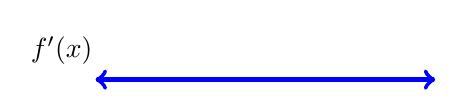
\begin{tikzpicture}
    \begin{axis}[
    	axis x line=none,
	            axis y line=none,
		x label style={anchor=west},
            xlabel={},
            xtick       = {0},
            xticklabels = {$c$},
            y label style={anchor=south},
            ylabel={},
            ytick       = {-6,-4,-2,2,4,6},
            yticklabels = {$-6$,$-4$,$-2$,$2$,$4$,$6$},
            samples     = 320,
            domain      = -2.5:2.5,
            restrict y to domain=-6.5:6.5,
            xmin = -3.5, xmax = 3.5,
            ymin = -6.5, ymax = 6.5,
            width=3in, height=2.5in,
            grid=none, grid style=solid
          ]
    \addplot[domain=-2.5:2.5, blue, ultra thick, mark=none, <->]{0)};
   \draw (-3,1) node{$\Large f^{\prime}(x)$};
%   \draw[ultra thick, blue] (0,.3)--(0,-.3);
%      \draw (0,-.6) node{$c$};
    \end{axis}
\end{tikzpicture}
}
\vs{1}
\item What, if anything, can we conclude from the First Derivative Test for Absolute Extrema? Do we have both an Absolute Max and an Absolute Min?
}

\newpage


{\bf\color{blue}Extra Practice 1.}\ltrm{\color{RedOrange}A2} Find the absolute extrema of $M(x)=2x-6\sqrt{x}$ on the interval $[0,\infty)$.
\vfill

{\bf\color{blue}Extra Practice 2.}\ltrm{\color{RedOrange}A2} Find the absolute extrema of $f(x)=x+\dfrac{16}{x}$ on the interval $(0,\infty)$.


\vfill

{\bf\color{blue}Extra Practice 3.}\ltrm{\color{RedOrange}A2} Find the absolute extrema of $f(x)=\dfrac{1}{x^2-2x+2}$ on the intervals below:\\[0.1in]
%
\,\hfill
%
\fbox{
\begin{minipage}{0.15\textwidth}
\begin{center}
{\Large$\left[-1,2\right]$}
\end{center}
max: \rule[-8pt]{0.5in}{0.4pt}\\[0.2in]
min: \,\rule[-8pt]{0.5in}{0.4pt}
\end{minipage}
}
%
\hfill
%
\fbox{
\begin{minipage}{0.15\textwidth}
\begin{center}
{\Large$\left[-1,2\right)$}
\end{center}
max: \rule[-8pt]{0.5in}{0.4pt}\\[0.2in]
min: \,\rule[-8pt]{0.5in}{0.4pt}
\end{minipage}
}
%
\hfill
%
\fbox{
\begin{minipage}{0.15\textwidth}
\begin{center}
{\Large$\left(-1,2\right]$}
\end{center}
max: \rule[-8pt]{0.5in}{0.4pt}\\[0.2in]
min: \,\rule[-8pt]{0.5in}{0.4pt}
\end{minipage}
}
%
\hfill
%
\fbox{
\begin{minipage}{0.15\textwidth}
\begin{center}
{\Large$\left(-1,2\right)$}
\end{center}
max: \rule[-8pt]{0.5in}{0.4pt}\\[0.2in]
min: \,\rule[-8pt]{0.5in}{0.4pt}
\end{minipage}
}
%
\hfill\,\\[0.2in]
%

\vfill

%%%%%%%%%
\newpage%
%%%%%%%%%

{\bf\color{blue}Extra Practice 4.}\ltrm{\color{RedOrange}A2} Let $f(x)=24\ln(x)+x^3$. Find the absolute extrema of $f(x)$ over $(0,3]$. ({\bf Hint:} do you recall what happens to the graph of the natural logarithmic function as its input approaches $0$ from the right?)

\end{document}
